% Body (at most 4 pages). Compiled by body.tex (alone) and main.tex (full proposal).
\begin{center}
\begin{large}
{\bf Feasibility study of an X17 search in \Li\pee\Be{}\\ with the MX17 Micromegas-TPC spectrometer}\\
\vspace{.2cm}
{\bf Experimental Setup: MX17, two-arm configuration}\\
\end{large}
\end{center}
\vspace{.4cm}
\begin{flushleft}
{\bf Spokesperson(s): \todo{to decide: D.~Neff / P.~Mastinu}}
\end{flushleft}
\thispagestyle{empty}
\pagestyle{empty}

% Body limit: the template says "should not exceed 4 pages" (the LNL web page says 5). Keep to 4.
% Prose rewritten 2026-11-24 in Dylan's style (nTof_x17/papers/WRITING_STYLE.md); numbers: sim2arm/TWO_ARM_STUDY.md §0,
% PREDICTIONS.md (Cu hemisphere dome300, pass 4); four-arm light-holder days: x17_facility_search FEASIBILITY_SIM §19.3.
\section{Scientific motivation}

In 2016 the ATOMKI group observed an excess of $e^+e^-$ pairs at large opening angles
($\theta \approx 140^\circ$) in the decay of the 18.15~MeV $J^\pi = 1^+$ state of \Be{}. This state is populated in
\Li$(p,\gamma)$ at $E_p \approx 1.04$~MeV~\cite{Kra16}. The excess is consistent with the emission of a
neutral boson with a mass $m_X \approx 16.7$~MeV and a branching ratio
$R = \Gamma_X/\Gamma_\gamma \approx 5.8\times10^{-6}$. We call this ratio $R_\mathrm{ATOMKI}$. Similar anomalies were
later reported in \textsuperscript{4}He and \textsuperscript{12}C~\cite{Kra21}, and in the \Be{} direct-capture
region~\cite{Sas22}. An independent two-arm spectrometer, built in Hanoi with ATOMKI, reported an excess of more than
$4\sigma$ at $E_p = 1.225$~MeV~\cite{Anh24}.

The MEG~II collaboration measured the same reaction with its large tracking detector and found no
signal. MEG~II sets $R(18.15) < 1.2\times10^{-5}$ at 90\,\% CL~\cite{MEG24}, which is $2.07\times R_\mathrm{ATOMKI}$. In 2026,
members of MEG~II simulated the ATOMKI spectrometers in full. They showed that cosmic-ray coincidences produce a
structure near $140^\circ$ in the \Be{} energy window, and that this structure is comparable to the internal pair
creation (IPC) itself at the ATOMKI running conditions~\cite{MEG26}. The question is therefore open. However, the
experimental requirements to settle it are clear. The lepton directions must be \emph{measured}. The rejection of cosmic
rays must be strong, and it must be \emph{demonstrated}. The angular response must be calibrated on a transition with no
anomaly. Finally, the acceptance must be large enough to reach the ATOMKI branching ratio with a margin. At LNL, a pair
spectrometer made of scintillator telescopes took data on AN2000 in 2023--24~\cite{GS25}. A measurement with tracking
would be complementary to it.
\todo{one sentence after talking to the LNL \Be{} group (T.~Marchi et al.)}

The MX17 apparatus was built to search for \Xs{} in $^3$He$(n,e^+e^-)^4$He at CERN n\_TOF, where it
took data in 2026~\cite{Gus20}. Each arm combines a Micromegas time projection chamber (TPC) with a scintillator wall and
plastic scintillators. The Micromegas TPC measures the lepton position to 0.6--0.8~mm, and the scintillators give the
trigger and the energy. On a low-energy proton beam this apparatus meets each requirement above. The opening angle is
reconstructed from the tracked hits. Cosmic muons are recognised by their straight tracks, which cross two arms. Four arms
cover about 40\,\% of the solid angle for the \Xs{} pairs. A full Geant4 simulation of four arms around a \Li{} target in
a light holder (an aluminium ogive with a thin copper liner) predicts a $3\sigma$ test of $R_\mathrm{ATOMKI}$ in about 5 to
9 days at 1~\si{\micro\ampere} with the apparatus as built. The range depends on the response of the liquid scintillator.
With large plastic scintillators the same test takes less than a day. The aim of the present proposal is to check the inputs of
this simulation on the beam, before we propose that measurement. These inputs are the rates, the backgrounds and the
detector response.

\section{The apparatus and the two-arm configuration}

\begin{figure}[tb]
\begin{minipage}[c]{0.62\textwidth}\centering
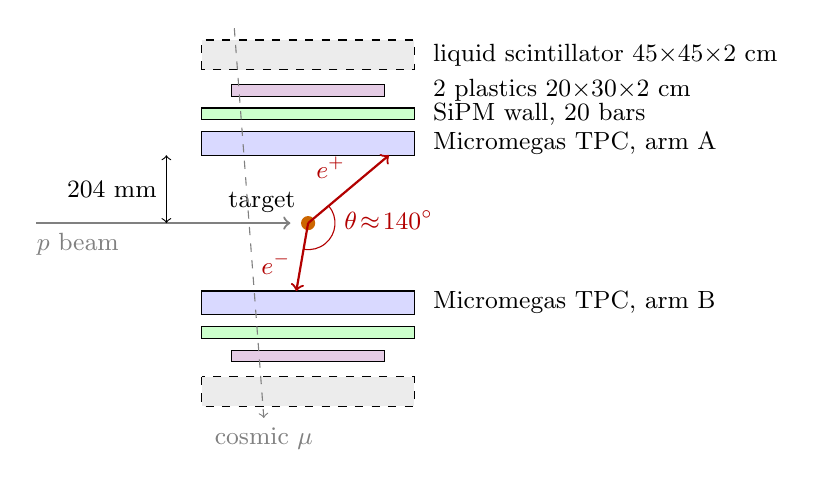
\begin{tikzpicture}[scale=0.75,font=\small]
  % beam
  \draw[->,thick,gray] (-4.6,0) -- (-0.3,0);
  \node[gray,below] at (-3.9,0) {$p$ beam};
  \fill[orange!80!black] (0,0) circle (0.12);
  \node[above left] at (-0.05,0.02) {\Li{} target};
  \foreach \s in {1,-1}{
    \begin{scope}[yscale=\s]
      \fill[blue!15] (-1.8,1.15) rectangle (1.8,1.55);  \draw (-1.8,1.15) rectangle (1.8,1.55);
      \fill[green!20] (-1.8,1.75) rectangle (1.8,1.95); \draw (-1.8,1.75) rectangle (1.8,1.95);
      \fill[violet!20] (-1.3,2.15) rectangle (1.3,2.35); \draw (-1.3,2.15) rectangle (1.3,2.35);
      \fill[gray!15] (-1.8,2.6) rectangle (1.8,3.1); \draw[dashed] (-1.8,2.6) rectangle (1.8,3.1);
    \end{scope}
  }
  \node[right] at (1.95,1.35) {Micromegas TPC, arm A};
  \node[right] at (1.95,1.85) {SiPM wall, 20 bars};
  \node[right] at (1.95,2.25) {2 plastics $20{\times}30{\times}2$~cm};
  \node[right] at (1.95,2.85) {liquid scintillator $45{\times}45{\times}2$~cm};
  \node[right] at (1.95,-1.35) {Micromegas TPC, arm B};
  % pair, opening angle 140 deg
  \draw[->,red!70!black,thick] (0,0) -- (1.37,1.15) node[pos=0.55,above left=-1pt]{$e^+$};
  \draw[->,red!70!black,thick] (0,0) -- (-0.2,-1.15) node[pos=0.6,left]{$e^-$};
  \draw[red!70!black] (0.35,0.29) arc (40:-100:0.45);
  \node[red!70!black,right] at (0.45,0.05) {$\theta\!\approx\!140^\circ$};
  % muon
  \draw[->,gray,dashed] (-1.25,3.3) -- (-0.75,-3.3) node[below]{cosmic $\mu$};
  \draw[<->] (-2.4,0) -- (-2.4,1.15) node[midway,left]{204~mm};
\end{tikzpicture}
\end{minipage}\hfill
\begin{minipage}[c]{0.36\textwidth}
\caption{The two-arm configuration, seen from above (not to scale). Each arm contains a Micromegas TPC
(30~mm drift, $399\times360$~mm$^2$ active area), a wall of 20 plastic bars read by SiPMs, two plastic
scintillators and a liquid scintillator cell. The two arms face each other across the beam, where the \Xs{} pairs
($\theta\approx135$--$140^\circ$) arrive. A cosmic muon crosses both arms on one straight line and is rejected.}
\label{fig:setup}
\end{minipage}
\end{figure}

\paragraph{Arms.} Figure~\ref{fig:setup} shows the two-arm configuration. Going outward from the beam axis, each arm
contains a Micromegas TPC, a wall of 20 EJ-212 bars read by SiPMs, two $20\times30\times2$~cm$^3$ plastic scintillators
read by PMTs, and a $45\times45\times2$~cm$^3$ liquid scintillator cell read by one PMT. The TPC has a 30~mm drift gap and
an aluminised-mylar window, and the faces of the two TPCs are at $\pm204$~mm from the beam. The liquid cell is a new
container filled with the liquid used at n\_TOF. The liquid measures the lepton energy that 2~cm of plastic does not absorb. In simulation, the running time
needed for the same sensitivity is 3.4 times longer without the liquid cells. Thicker cells (4~cm, or two 2~cm cells in
series) are being studied. The two Micromegas chosen for this run reached 91--93\,\% efficiency within 5~mm on a cosmic
bench in 2026. One of them needs a repair of its drift window, which CEA Saclay will do in spring 2027.

\paragraph{Readout and trigger.} The Micromegas are read by the DREAM system of CEA, with 4 front-end units and the trigger
and clock unit for the two arms. The scintillators are recorded on about 24 digitizer channels: 16 sums of the SiPM wall,
4--6 PMTs and a trigger word. We use the trigger of the n\_TOF run. Each arm forms a leg from its wall and its plastics in
a 20~ns coincidence. A PAIR trigger requires a leg in both arms, and it is never prescaled. SINGLE triggers (a leg in one
arm) are prescaled by $P = 10$--50 and are used to monitor the gains. A 1~Hz clock trigger is also recorded. The busy
signal of DREAM vetoes the trigger, so that both systems record the same list of events. At the LNL rates DREAM is more
than 95\,\% live.

\paragraph{Target.} The target is a thin metallic lithium film, 10--12~\si{\micro\metre} thick. The film is rolled and
pressed onto a backing in the argon glovebox of the LNL CN target laboratory. It sits at the apex of the existing copper hemisphere that closes the beam line
(radius 11~mm, 300~\si{\micro\metre} wall). This wall costs most of the sensitivity. Every lepton crosses 2\,\% $X_0$ of copper, or the thicker rim, so it loses
about 1~MeV and scatters by about 10$^\circ$. In simulation, a lighter aluminium end piece (an aluminium ogive with a thin copper liner, or a flat aluminium end cap
at 45$^\circ$) reduces the running time needed by about an order of magnitude. An optimised holder is being studied at
LNL. \todo{whether one can be ready for this run.}
A 10--12~\si{\micro\metre} film is thin enough that the 1.10~MeV beam does not slow down to the 441~keV resonance inside
the film, even after part of the lithium has turned into LiOH. The lithium must be free of boron, since $^{11}$B$(p,\gamma)$ produces
$\gamma$ rays of 16--17~MeV.

\section{Measurements and expected precision}

The run consists of four measurements. Each one tests Geant4 predictions of inputs to the expected limit, and
Table~\ref{tab:pred} lists these predictions. The run compares each prediction with the data.
\begin{enumerate}[leftmargin=1.5em]
\item \textbf{Rates and live time.} We scan the beam current from 0.05 to 1~\si{\micro\ampere} at 1.10~MeV. At each
current we measure the single-arm and two-arm trigger rates, the live time of DREAM, the occupancy and noise of the
Micromegas, and the beam-induced singles in the scintillators. Every leg has a scaler, so each rate is known to better
than 1\,\% (statistical) in a few minutes.
\item \textbf{Calibration on the 17.64~MeV M1 transition} ($E_p = 441$~keV, $\Gamma_\mathrm{lab} = 12$~keV,
$\sigma \approx 5.9$~mb). ATOMKI saw no anomaly at this resonance. For this reason the IPC distribution here serves as a
calibration. The Geant4 simulation of the two arms with the Cu hemisphere gives about 140 selected pairs per day above
$90^\circ$ at 1~\si{\micro\ampere} (about 1600 without the cut on the energy sum). In one day we therefore measure the
absolute pair rate to about 8\,\%. We also compare the opening-angle distribution with Geant4, and we fix the energy scale
from the summed energy.
\item \textbf{Backgrounds.} Before the beam days, we run a few nights of cosmic rays with the two arms stacked vertically.
In this orientation the cosmic rays reproduce, at full strength, the $140^\circ$ structure at the core of the 2026
critique of ATOMKI-type spectrometers~\cite{MEG26}. The simulation gives about $1.6\times10^5$ two-arm coincidences per
day, and half of them fall at 125--$160^\circ$. These nights measure how much each veto (the track pointing and the
arm-to-arm time of flight) rejects, and they measure the time-of-flight resolution itself. For the beam days the arms are
horizontal. In this orientation the simulation gives about 25 times fewer cosmic coincidences. The beam-on runs measure the
accidental coincidences and the external pair conversions. Half a day with the arms at $90^\circ$ to each other measures
the external conversions at 25--$90^\circ$ (several thousand per day).
\item \textbf{The 18.15~MeV region} ($E_p = 1.10$~MeV, five days). For a 300~\si{\micro\gram\per\centi\metre\squared}
Li$_2$O film (the ATOMKI conditions), the rates are about $2\times10^3$ ground-state $\gamma$ rays per second and about 7
IPC pairs per second into $4\pi$, per \si{\micro\ampere}. A 10--12~\si{\micro\metre} metallic film gives about 4--5 times
more. We fit the opening angle, the energy sharing and the energy sum together. In this fit the shape of the background is
free within the limits set by the calibration. Figure~\ref{fig:reach} shows the expected limit from the full Geant4
simulation of the two arms with the Cu hemisphere and 10--12~\si{\micro\metre} of lithium. In five days the expected
90\,\% CL limit is $R \lesssim 2.35\times R_\mathrm{ATOMKI}$ with the liquid cells. It is $3.1\times R_\mathrm{ATOMKI}$
if the liquid response is as it was at n\_TOF, and $4.3\times R_\mathrm{ATOMKI}$ with the SiPM walls and plastics alone.
For comparison, the MEG~II limit is $2.07\times R_\mathrm{ATOMKI}$. With a lighter aluminium end piece, the same five days
would give about 0.6--0.8$\times R_\mathrm{ATOMKI}$ (an estimate scaled from the four-arm simulation). This run therefore
tests the method and the backgrounds, and it sets a first limit. The full experiment (four arms, a light holder, large
plastics) is designed for a discovery-level test.
\end{enumerate}

\begin{table}[h]
\centering\footnotesize
\begin{tabular}{lll}
\toprule
observable & Geant4 prediction & what it checks \\
\midrule
cosmic PAIR triggers, arms vertical & 1.9~Hz ($7\times10^4$ per night) & veto at full strength \\
\quad with tracks in 2 / 1 / 0 arms & 84 / 15 / 0.7\,\% & chamber efficiency in situ \\
\quad at 125--$160^\circ$; wall-to-wall $\Delta t$ & 57\,\%; $+2.3$~ns, all downward & the $140^\circ$ structure; $\sigma_t$ \\
cosmic PAIR triggers, arms horizontal & 0.075~Hz (25$\times$ fewer) & orientation of the beam days \\
single-arm legs, per \si{\micro\ampere} & 218~Hz (441~keV), 67~Hz (1.10~MeV) & Li yield, holder wall \\
\quad with a Micromegas track & 72\,\% / 71\,\% & conversions in the Cu wall \\
two-track pairs per day, all $\theta$ & 9000 (441~keV), 3300 (1.10~MeV) & acceptance, live time \\
selected pairs per day ($\theta>90^\circ$) & 141 (441~keV), 69 (1.10~MeV) & IPC rate and shape, $E$ scale \\
\quad of which external conversions & 1 / 17 & holder model \\
selected cosmic pairs per day & 68 & veto with beam \\
\Xs{} at $R_\mathrm{ATOMKI}$, selected per day & 2.7 (1.10~MeV) & the sensitivity above \\
\bottomrule
\end{tabular}
\caption{Geant4 predictions for the run, two horizontal arms (vertical where stated), the Cu hemisphere, 11~\si{\micro\metre}
Li, 1~\si{\micro\ampere}, chamber efficiency 0.92. A selected pair has an energy sum of 13--19~MeV, tracks that point to the
target and a time of flight within 0.6~ns.}
\label{tab:pred}
\end{table}

\begin{figure}[t]
\begin{minipage}[c]{0.6\textwidth}
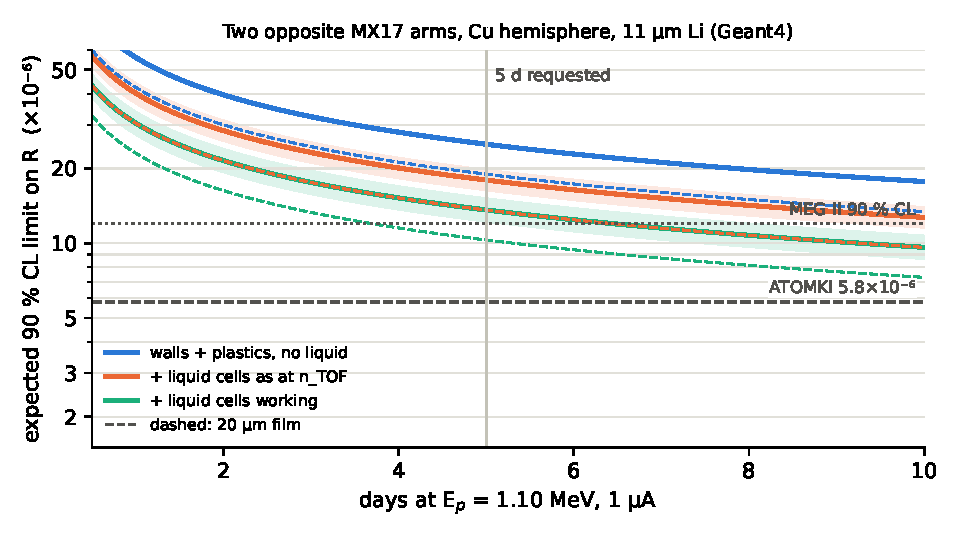
\includegraphics[width=\textwidth]{figures/limit_vs_days.pdf}
\end{minipage}\hfill
\begin{minipage}[c]{0.38\textwidth}
\caption{Expected 90\,\% CL upper limit on $R=\Gamma_X/\Gamma_\gamma$ as a function of the number of days at
$E_p=1.10$~MeV and 1~\si{\micro\ampere}. The set-up is two opposite arms (horizontal), the existing Cu hemisphere and
11~\si{\micro\metre} of Li (dashed lines: 20~\si{\micro\metre}). The three colours are three calorimeter configurations.
The limits come from Geant4, with cosmic rays, and a fit in which the background shape floats. The bands span two
estimators of the Monte Carlo statistics.}
\label{fig:reach}
\end{minipage}
\end{figure}

\section{Beam-time request}

\begin{table}[h]
\centering\footnotesize
% Only l columns: revtex4 (2001) breaks on p{} and @{} with the array package of current TeX Live (Overleaf).
\newcommand{\daycell}[1]{\parbox[t]{0.78\textwidth}{\raggedright #1\strut}}
\begin{tabular}{lll}
\toprule
day & $E_p$ & measurement \\
\midrule
before & -- & \daycell{installation nights, arms vertical: cosmic-ray rejection and time of flight} \\
1 & 1.10 MeV & \daycell{arms horizontal; target conditioning; current scan 0.05--1~\si{\micro\ampere}: rates, live time, occupancy} \\
2 & 0.441 MeV & \daycell{resonance located; 17.64~MeV IPC calibration, $\sim$140 pairs above $90^\circ$} \\
3--7 & 1.10 MeV & \daycell{18.15~MeV region; daily $\gamma$-yield check of the target} \\
8 & 1.10 MeV & \daycell{half a day with the arms at $90^\circ$ (external conversions); contingency} \\
\bottomrule
\end{tabular}
\caption{Use of the 8 days requested. The beam is protons, continuous, at most 1~\si{\micro\ampere}, at two energies.
There is at most one energy change per day, which suits the self-service operation of AN2000.}
\label{tab:days}
\end{table}

We request \textbf{8 days of proton beam on AN2000} in the second half of 2027. Table~\ref{tab:days} shows how the days
are used. The beam line should end in about $1.5\times1.5$~m$^2$ of free floor around the target. The CN could run the
1.10~MeV programme. However, it cannot run the 441~keV calibration, which is below its minimum of 0.8~MV.
\todo{line, floor, 24 h operation: confirm with the Accelerator Division.}

\section{From feasibility to the full experiment; requirements}

The calibration, the measured backgrounds and the timing between the arms will replace the corresponding inputs of the
simulation. With these inputs we will fix the design of the full experiment. This experiment has four arms and larger
calorimeter legs. In simulation, large plastic scintillators reduce the running time by a factor of 13--15. As an
alternative, we are studying wider and thicker liquid cells made from the $\sim$60~L of liquid available. The programme
includes beam energies on and off the resonance (0.80, 1.10 and 1.225~MeV), and it will be the subject of a later proposal.

\textbf{Requirements and safety.} The Micromegas use premixed Ar/iC$_4$H$_{10}$ (95/5) at about 1~L/h, with an exhaust.
Whether this mixture is below the flammability limit is still to be checked. \todo{LNL rules} The Micromegas need at most
600~V, and the PMTs and the SiPM bias use standard supplies. The metallic lithium is handled in the CN
target laboratory. The equipment is owned by the collaboration or lent by CEA and INFN. The installation starts
\todo{weeks} before the beam days.

\vspace{-0.6cm}
\begin{thebibliography}{999}\footnotesize
\setlength{\itemsep}{0pt}
\bibitem{Kra16} A.J.~Krasznahorkay \emph{et al.}, Phys.\ Rev.\ Lett.\ \textbf{116}, 042501 (2016).
\bibitem{Kra21} A.J.~Krasznahorkay \emph{et al.}, Phys.\ Rev.\ C \textbf{104}, 044003 (2021); review: arXiv:2409.16300 (2024).
\bibitem{Sas22} N.J.~Sas \emph{et al.}, arXiv:2205.07744 (2022).
\bibitem{Anh24} Tran The Anh \emph{et al.}, arXiv:2401.11676 (2024).
\bibitem{MEG24} MEG~II Collaboration, K.~Afanaciev \emph{et al.}, arXiv:2411.07994. \todo{journal ref}
\bibitem{MEG26} H.~Benmansour \emph{et al.}, arXiv:2609.18383 (2026).
\bibitem{GS25} B.~Góngora-Servín \emph{et al.}, Acta Phys.\ Pol.\ B Proc.\ Suppl.\ \textbf{18}, 2-A13 (2025).
\bibitem{Gus20} C.~Gustavino \emph{et al.}, \Xs{} at n\_TOF proposal \todo{CERN-INTC reference}.
\end{thebibliography}
